\section{Теоретические сведения}
\addcontentsline{toc}{section}{Теоретические сведения}	% Добавляем его в оглавление

Инструментальная погрешность имеет различные формы: абсолютную ($ \Delta $), относительную ($ \delta $) и приведённую ($ \gamma $):

\begin{equation*}
  \label{eq:equation1}
  \Delta_{i} = \vert X_{i} - Q \vert
\end{equation*}

\begin{equation*}
  \label{eq:equation2}
  \delta_{i} = \dfrac{\Delta_{i}}{Q} * 100\% = \gamma_{i} * \dfrac{X_{N}}{Q}
\end{equation*}

\begin{equation*}
  \label{eq:equation3}
  \gamma_{i} = \dfrac{\Delta_{i}}{X_{N}}*100\%
\end{equation*}

\noindent где $ X_{N} $ -- нормируемое значение, которое согласно ГОСТ 8.401-80 следует выбирать равным пределу измерения,

$ Q $ -- действительное значение величины,

$ X_{i} $ -- показание прибора.

\vspace{4mm}

Входное сопротивление $ R_{V} $ и входная емкость $ C_{V} $ вольтметра B7-28 определяется по следующим формулам:

\begin{equation*}
  \label{eq:equation4}
  R_{V} = R_{0} * \dfrac{U_{R_{V}} - 1}{U_{G_{H}}}
\end{equation*}

\begin{equation*}
  \label{eq:equation5}
  C_{V} = C_{0} * ( \dfrac{U_{G_{B}}}{U_{C_{V}}} - 1)
\end{equation*}

\noindent где $ R_{V} $ -- активное сопротивление,\par
$ C_{V} $ -- входная емкость,\par
$ U_{C_{V}} $, $ U_{R_{V}} $ -- показания вольтметра,\par
$ U_{G_{H}} $ -- напряжение генератора на нижней частоте,\par
$ U_{G_{B}} $ -- напряжение генератора на верхней частоте,\par
$ C_{0} $, $ R_{0} $ -- известные сопротивление и емкость, включенные в схему.\par

\vspace{4mm}

Коэффициенты амплитуды $ K_{a} $ и формы $ K_{f} $ рассчитываются по формулам:

\begin{equation*}
  \label{eq:equation6}
  K_{f} = \dfrac{U_{CK}}{U_{CB}}
\end{equation*}

\begin{equation*}
  \label{eq:equation4}
  R_{a} = \dfrac{U_{m}}{U_{CK}}
\end{equation*}

\begin{figure}[h]
  \center{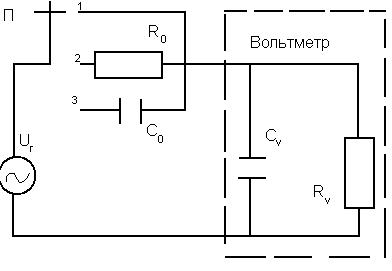
\includegraphics[width=0.8\linewidth]{scheme1}}
  \caption{Принципиальная схема установки}
\end{figure}


\vspace{4mm}

\begin{table} [htbp]
  \begin{center}
    \begin{tabular}{ p{5cm} p{5cm} p{5cm}l }

      \centering B4-12 \par &\centering B3-40 &\centering B3-38 & \\
      \centering $ U_{m} = U_{V} $ \par &\centering $ U_{CK} = U_{V} $ &\centering $ U_{CB} = U_{V}/1.11 $ & \\
      \centering $ \delta_{B4-12} = \gamma * \dfrac{U_{pr. B4-12}}{U_{B4-12}} $ \par
      &\centering $ \delta_{B3-40} = \gamma * \dfrac{U_{pr. B3-40}}{U_{B3-40}} $ 
      &\centering $ \delta_{B3-38} = \gamma * \dfrac{U_{pr. B3-38}}{U_{B3-38}}$ & \\

      \centering $ \gamma = \pm 4 \% $ &\centering $ \gamma = \pm 1,5 \% $ \par &\centering $ \gamma = \pm 2,5 \% $ \\ 

    \end{tabular}
  \end{center}
\end{table}



\clearpage
